\documentclass{standalone}
\usepackage{tikz}
\usetikzlibrary{patterns, positioning}

\begin{document}
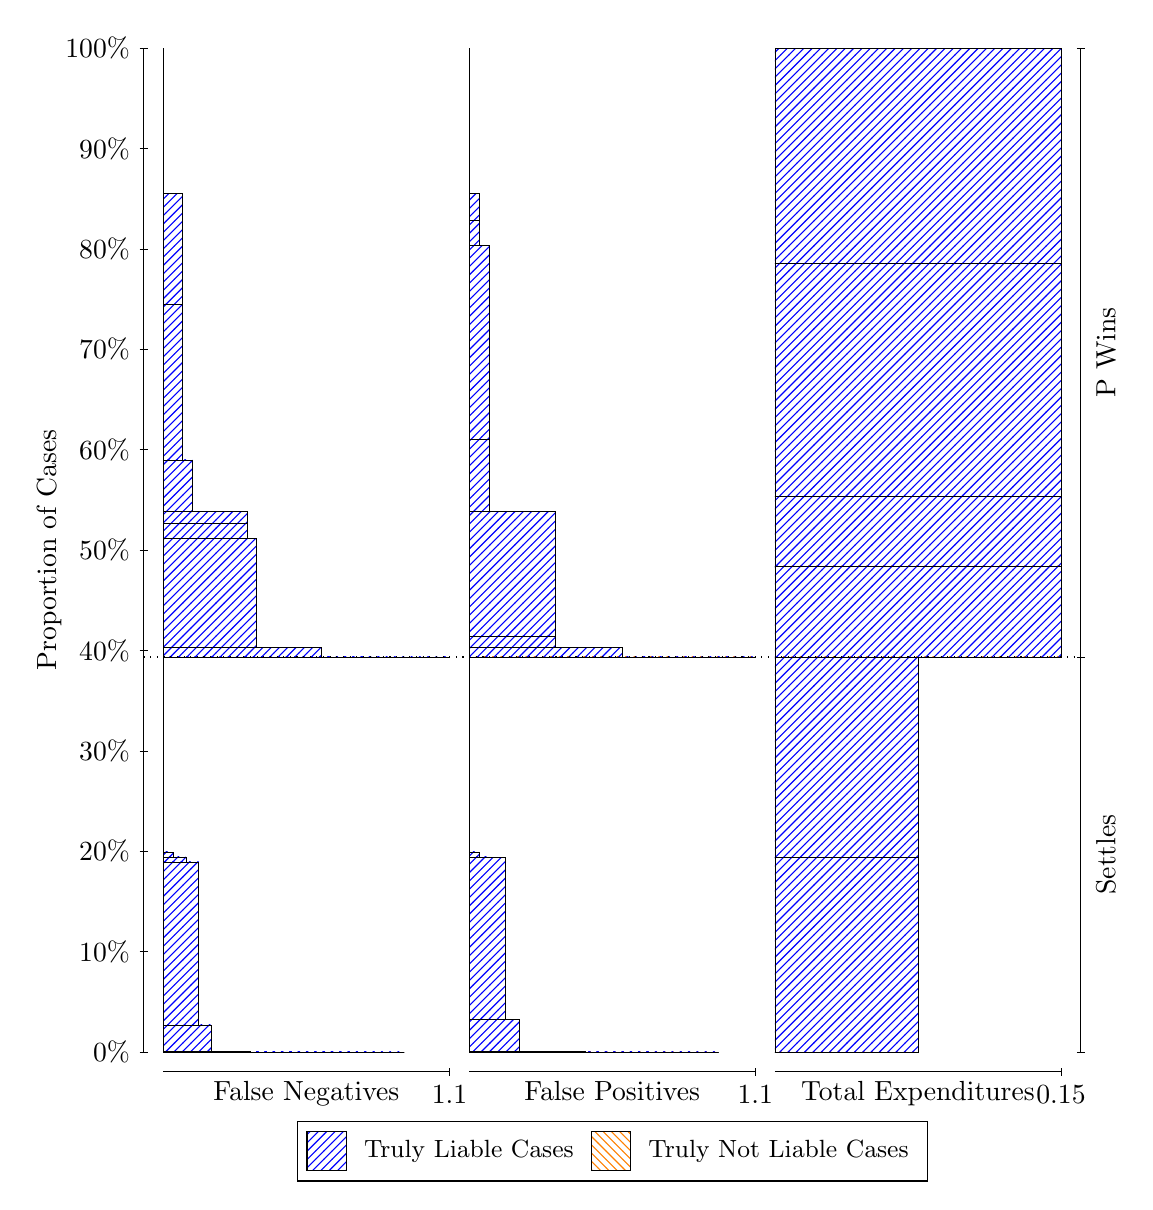
\begin{tikzpicture}
\draw[black, very thin] (1.5,1.75) -- (1.5,14.5);
\node[rotate=90, anchor=center] at (0.3, 8.125) {Proportion of Cases};
\draw[black, very thin] (1.45,1.75) -- (1.55,1.75);
\node[anchor=east] at (1.45, 1.75) {0\%};
\draw[black, very thin] (1.45,3.025) -- (1.55,3.025);
\node[anchor=east] at (1.45, 3.025) {10\%};
\draw[black, very thin] (1.45,4.3) -- (1.55,4.3);
\node[anchor=east] at (1.45, 4.3) {20\%};
\draw[black, very thin] (1.45,5.575) -- (1.55,5.575);
\node[anchor=east] at (1.45, 5.575) {30\%};
\draw[black, very thin] (1.45,6.85) -- (1.55,6.85);
\node[anchor=east] at (1.45, 6.85) {40\%};
\draw[black, very thin] (1.45,8.125) -- (1.55,8.125);
\node[anchor=east] at (1.45, 8.125) {50\%};
\draw[black, very thin] (1.45,9.4) -- (1.55,9.4);
\node[anchor=east] at (1.45, 9.4) {60\%};
\draw[black, very thin] (1.45,10.675) -- (1.55,10.675);
\node[anchor=east] at (1.45, 10.675) {70\%};
\draw[black, very thin] (1.45,11.95) -- (1.55,11.95);
\node[anchor=east] at (1.45, 11.95) {80\%};
\draw[black, very thin] (1.45,13.225) -- (1.55,13.225);
\node[anchor=east] at (1.45, 13.225) {90\%};
\draw[black, very thin] (1.45,14.5) -- (1.55,14.5);
\node[anchor=east] at (1.45, 14.5) {100\%};

\draw[black, very thin] (13.4,1.75) -- (13.4,14.5);
\draw[black, very thin] (13.35,1.75) -- (13.45,1.75);
\node[anchor=west] at (13.35, 1.75) {};
\draw[black, very thin] (13.35,6.7663) -- (13.45,6.7663);
\node[anchor=west] at (13.35, 6.7663) {};
\draw[black, very thin] (13.35,14.5) -- (13.45,14.5);
\node[anchor=west] at (13.35, 14.5) {};

\draw[black, very thin, pattern color=blue, pattern=north east lines] (1.75,1.75) rectangle (4.8118,1.75);
\draw[black, very thin, pattern color=blue, pattern=north east lines] (1.75,1.75) rectangle (4.4852,1.75);
\draw[black, very thin, pattern color=blue, pattern=north east lines] (1.75,1.75) rectangle (4.1586,1.75);
\draw[black, very thin, pattern color=blue, pattern=north east lines] (1.75,1.75) rectangle (3.9953,1.75);
\draw[black, very thin, pattern color=blue, pattern=north east lines] (1.75,1.75) rectangle (3.6687,1.75);
\draw[black, very thin, pattern color=blue, pattern=north east lines] (1.75,1.75) rectangle (3.5054,1.75);
\draw[black, very thin, pattern color=blue, pattern=north east lines] (1.75,1.75) rectangle (3.3421,1.75);
\draw[black, very thin, pattern color=blue, pattern=north east lines] (1.75,1.75) rectangle (3.1788,1.7505);
\draw[black, very thin, pattern color=blue, pattern=north east lines] (1.75,1.7505) rectangle (2.8522,1.7529);
\draw[black, very thin, pattern color=blue, pattern=north east lines] (1.75,1.7529) rectangle (2.689,1.7553);
\draw[black, very thin, pattern color=blue, pattern=north east lines] (1.75,1.7553) rectangle (2.5257,1.7558);
\draw[black, very thin, pattern color=blue, pattern=north east lines] (1.75,1.7558) rectangle (2.3624,2.0937);
\draw[black, very thin, pattern color=blue, pattern=north east lines] (1.75,2.0937) rectangle (2.1991,4.1627);
\draw[black, very thin, pattern color=blue, pattern=north east lines] (1.75,4.1627) rectangle (2.0358,4.1633);
\draw[black, very thin, pattern color=blue, pattern=north east lines] (1.75,4.1633) rectangle (2.0358,4.2265);
\draw[black, very thin, pattern color=blue, pattern=north east lines] (1.75,4.2265) rectangle (1.8725,4.2897);
\draw[black, very thin, pattern color=orange, pattern=north west lines] (1.75,4.2897) rectangle (1.75,4.2897);
\draw[black, very thin, pattern color=blue, pattern=north east lines] (1.75,4.2897) rectangle (1.75,6.7663);
\draw[black, very thin, pattern color=blue, pattern=north east lines] (1.75,6.7663) rectangle (5.3833,6.7663);
\draw[black, very thin, pattern color=blue, pattern=north east lines] (1.75,6.7663) rectangle (4.5669,6.7675);
\draw[black, very thin, pattern color=blue, pattern=north east lines] (1.75,6.7675) rectangle (4.4444,6.7675);
\draw[black, very thin, pattern color=blue, pattern=north east lines] (1.75,6.7675) rectangle (3.7504,6.8861);
\draw[black, very thin, pattern color=blue, pattern=north east lines] (1.75,6.8861) rectangle (3.6279,6.8863);
\draw[black, very thin, pattern color=blue, pattern=north east lines] (1.75,6.8863) rectangle (2.9339,8.2774);
\draw[black, very thin, pattern color=blue, pattern=north east lines] (1.75,8.2774) rectangle (2.8114,8.4655);
\draw[black, very thin, pattern color=blue, pattern=north east lines] (1.75,8.4655) rectangle (2.8114,8.6133);
\draw[black, very thin, pattern color=blue, pattern=north east lines] (1.75,8.6133) rectangle (2.1174,9.2707);
\draw[black, very thin, pattern color=blue, pattern=north east lines] (1.75,9.2707) rectangle (1.9949,11.248);
\draw[black, very thin, pattern color=blue, pattern=north east lines] (1.75,11.248) rectangle (1.9949,12.653);
\draw[black, very thin, pattern color=orange, pattern=north west lines] (1.75,12.653) rectangle (1.75,12.653);
\draw[black, very thin, pattern color=blue, pattern=north east lines] (1.75,12.653) rectangle (1.75,14.5);
\draw[black, very thin, pattern color=orange, pattern=north west lines] (5.6333,1.75) rectangle (8.8019,1.75);
\draw[black, very thin, pattern color=blue, pattern=north east lines] (5.6333,1.75) rectangle (8.8019,1.75);
\draw[black, very thin, pattern color=orange, pattern=north west lines] (5.6333,1.75) rectangle (8.126,1.75);
\draw[black, very thin, pattern color=blue, pattern=north east lines] (5.6333,1.75) rectangle (8.126,1.75);
\draw[black, very thin, pattern color=blue, pattern=north east lines] (5.6333,1.75) rectangle (7.957,1.75);
\draw[black, very thin, pattern color=orange, pattern=north west lines] (5.6333,1.75) rectangle (7.45,1.75);
\draw[black, very thin, pattern color=blue, pattern=north east lines] (5.6333,1.75) rectangle (7.45,1.75);
\draw[black, very thin, pattern color=blue, pattern=north east lines] (5.6333,1.75) rectangle (7.281,1.75);
\draw[black, very thin, pattern color=blue, pattern=north east lines] (5.6333,1.75) rectangle (7.112,1.7529);
\draw[black, very thin, pattern color=orange, pattern=north west lines] (5.6333,1.7529) rectangle (6.774,1.7529);
\draw[black, very thin, pattern color=blue, pattern=north east lines] (5.6333,1.7529) rectangle (6.774,1.7529);
\draw[black, very thin, pattern color=blue, pattern=north east lines] (5.6333,1.7529) rectangle (6.605,1.7553);
\draw[black, very thin, pattern color=orange, pattern=north west lines] (5.6333,1.7553) rectangle (6.436,1.7553);
\draw[black, very thin, pattern color=blue, pattern=north east lines] (5.6333,1.7553) rectangle (6.436,1.7586);
\draw[black, very thin, pattern color=blue, pattern=north east lines] (5.6333,1.7586) rectangle (6.436,1.7591);
\draw[black, very thin, pattern color=blue, pattern=north east lines] (5.6333,1.7591) rectangle (6.2671,2.1603);
\draw[black, very thin, pattern color=orange, pattern=north west lines] (5.6333,2.1603) rectangle (6.0981,2.1603);
\draw[black, very thin, pattern color=blue, pattern=north east lines] (5.6333,2.1603) rectangle (6.0981,4.2261);
\draw[black, very thin, pattern color=blue, pattern=north east lines] (5.6333,4.2261) rectangle (5.9291,4.2266);
\draw[black, very thin, pattern color=blue, pattern=north east lines] (5.6333,4.2266) rectangle (5.7601,4.2898);
\draw[black, very thin, pattern color=blue, pattern=north east lines] (5.6333,4.2898) rectangle (5.6333,6.7663);
\draw[black, very thin, pattern color=orange, pattern=north west lines] (5.6333,6.7663) rectangle (9.2667,6.7663);
\draw[black, very thin, pattern color=blue, pattern=north east lines] (5.6333,6.7663) rectangle (9.2667,6.7663);
\draw[black, very thin, pattern color=orange, pattern=north west lines] (5.6333,6.7663) rectangle (8.4217,6.7663);
\draw[black, very thin, pattern color=blue, pattern=north east lines] (5.6333,6.7663) rectangle (8.4217,6.7675);
\draw[black, very thin, pattern color=orange, pattern=north west lines] (5.6333,6.7675) rectangle (7.5767,6.7675);
\draw[black, very thin, pattern color=blue, pattern=north east lines] (5.6333,6.7675) rectangle (7.5767,6.8863);
\draw[black, very thin, pattern color=orange, pattern=north west lines] (5.6333,6.8863) rectangle (7.45,6.8863);
\draw[black, very thin, pattern color=blue, pattern=north east lines] (5.6333,6.8863) rectangle (7.45,6.8863);
\draw[black, very thin, pattern color=orange, pattern=north west lines] (5.6333,6.8863) rectangle (6.7318,6.8863);
\draw[black, very thin, pattern color=blue, pattern=north east lines] (5.6333,6.8863) rectangle (6.7318,7.0338);
\draw[black, very thin, pattern color=blue, pattern=north east lines] (5.6333,7.0338) rectangle (6.7318,8.613);
\draw[black, very thin, pattern color=orange, pattern=north west lines] (5.6333,8.613) rectangle (6.605,8.613);
\draw[black, very thin, pattern color=blue, pattern=north east lines] (5.6333,8.613) rectangle (6.605,8.6133);
\draw[black, very thin, pattern color=blue, pattern=north east lines] (5.6333,8.6133) rectangle (5.8868,9.5287);
\draw[black, very thin, pattern color=blue, pattern=north east lines] (5.6333,9.5287) rectangle (5.8868,11.996);
\draw[black, very thin, pattern color=orange, pattern=north west lines] (5.6333,11.996) rectangle (5.7601,11.996);
\draw[black, very thin, pattern color=blue, pattern=north east lines] (5.6333,11.996) rectangle (5.7601,12.314);
\draw[black, very thin, pattern color=blue, pattern=north east lines] (5.6333,12.314) rectangle (5.7601,12.653);
\draw[black, very thin, pattern color=blue, pattern=north east lines] (5.6333,12.653) rectangle (5.6333,14.5);
\draw[black, very thin, pattern color=orange, pattern=north west lines] (9.5167,1.75) rectangle (11.333,1.75);
\draw[black, very thin, pattern color=blue, pattern=north east lines] (9.5167,1.75) rectangle (11.333,4.2232);
\draw[black, very thin, pattern color=orange, pattern=north west lines] (9.5167,4.2232) rectangle (11.333,4.2232);
\draw[black, very thin, pattern color=blue, pattern=north east lines] (9.5167,4.2232) rectangle (11.333,6.7663);
\draw[black, very thin, pattern color=orange, pattern=north west lines] (9.5167,6.7663) rectangle (13.15,6.7663);
\draw[black, very thin, pattern color=blue, pattern=north east lines] (9.5167,6.7663) rectangle (13.15,7.9222);
\draw[black, very thin, pattern color=orange, pattern=north west lines] (9.5167,7.9222) rectangle (13.15,7.9222);
\draw[black, very thin, pattern color=blue, pattern=north east lines] (9.5167,7.9222) rectangle (13.15,8.8015);
\draw[black, very thin, pattern color=orange, pattern=north west lines] (9.5167,8.8015) rectangle (13.15,8.8015);
\draw[black, very thin, pattern color=blue, pattern=north east lines] (9.5167,8.8015) rectangle (13.15,11.766);
\draw[black, very thin, pattern color=orange, pattern=north west lines] (9.5167,11.766) rectangle (13.15,11.766);
\draw[black, very thin, pattern color=blue, pattern=north east lines] (9.5167,11.766) rectangle (13.15,14.5);
\draw[black, dotted] (1.5,6.7663) -- (13.4,6.7663);
\draw[black, very thin] (1.75,1.5) -- (5.3833,1.5);
\node[anchor=north] at (3.5667, 1.5) {False Negatives};
\draw[black, very thin] (5.3833,1.45) -- (5.3833,1.55);
\node[anchor=north] at (5.3833, 1.45) {1.1};

\draw[black, very thin] (5.6333,1.5) -- (9.2667,1.5);
\node[anchor=north] at (7.45, 1.5) {False Positives};
\draw[black, very thin] (9.2667,1.45) -- (9.2667,1.55);
\node[anchor=north] at (9.2667, 1.45) {1.1};

\draw[black, very thin] (9.5167,1.5) -- (13.15,1.5);
\node[anchor=north] at (11.333, 1.5) {Total Expenditures};
\draw[black, very thin] (13.15,1.45) -- (13.15,1.55);
\node[anchor=north] at (13.15, 1.45) {0.15};

\node[black, centered, rotate=90] at (13.72, 4.2581) {Settles};
\node[black, centered, rotate=90] at (13.72, 10.633) {P Wins};

\draw (7.449999999999999,1.5) node[draw=none] (baseCoordinate) {};
\begin{scope}[align=center]
        \matrix[scale=0.5, draw=black, below=0.5cm of baseCoordinate, nodes={draw}, column sep=0.1cm]{
            \node[rectangle, draw, minimum width=0.5cm, minimum height=0.5cm, pattern=north east lines, pattern color=blue] {}; &
            \node[draw=none, font=\small] (B) {Truly Liable Cases}; &
            \node[rectangle, draw, minimum width=0.5cm, minimum height=0.5cm, pattern=north west lines, pattern color=orange] {}; &
            \node[draw=none, font=\small] (B) {Truly Not Liable Cases}; \\
            };
\end{scope}

\end{tikzpicture}
\end{document}